\documentclass[11pt,a4paper]{article}
\usepackage[utf8]{inputenc}
\usepackage{amsmath}
\usepackage{amsfonts}
\usepackage{amssymb}
\usepackage{makeidx}
\usepackage{graphicx}
\usepackage{lmodern}
\usepackage{kpfonts}
\usepackage{xcolor}
\usepackage{cancel}
\usepackage{mathtools}
\usepackage{schemata}
\usepackage{cancel}
\providecommand{\abs}[1]{\lvert#1\rvert}%Sirve para colocar valores absolutos
\providecommand{\norm}[1]{\lVert#1\rVert}%Sirve para colocar módulo
\usepackage[left=2.00cm, right=2.00cm, top=2.00cm,bottom=2.00cm]{geometry}
\author{Harold Alessander Jhon Zambrano Quispe}
\title{SOLUCIONARIO DE LA TAREA 1}
\begin{document}
   \begin{titlepage}%Habilita una pagina sin enumerar.
	\begin{center}
	 {\huge \textbf{Universidad Nacional de Ingeniería}}\\
	 \vspace{3mm}
	  {\Large {Facultad de Ingeniería Eléctrica y Electrónica}}\\
	\vspace{-5mm}	 
	 \begin{figure}[h]
	 	\centering 
	 	
\includegraphics[scale=0.5]{Logo UNI}
	 \end{figure}
	 \vspace{-6mm}
	{\Large {Especialidad de Ingeniería de Telecomunicaciones}}\\
	\vspace{3mm}
	{\Large \textbf{"Laboratorio 1 de Análisis de Señales y Sistemas"}}\\
	\vspace{8mm}
	\begin{flushleft}
	{\Large {\textbf{Curso}: Análisis de Señales y Sistemas}}\\
	\vspace{8mm}		
	{\Large {\textbf{Código del Curso}: EE410-M}}\\	
	\vspace{8mm}	
	{\Large {\textbf{Docente}: Manuel Arevalo Villanueva}}\\
	\vspace{8mm}	
	{\Large {\textbf{Integrantes}: 
	Gian Carlos Chancavilcas Osores - 20191108K\\
	\vspace{4mm}
	\hspace{3cm}Julio Cesar Luna Yabarrena - 20130346I\\ 
	\vspace{4mm}
	\hspace{3cm}Harold Alessander Jhon Zambrano Quispe - 20191351B}}\\
	\vspace{8mm}	
	\end{flushleft}
	\vspace{10mm}
	{\Huge {\textbf{2021-I}}}\\
	\end{center}
\end{titlepage}
%Se debe compilar desde la funcion principal
	\section{{\large \textbf{2. Sea $f[n]=3$ , $0\leq n \leq 2$, un pulso cuadrado , $g[n]=[1,2,3,2,1]$ un pulso triangular , sea $h[n]=(\frac{1}{2})^n$ , $0\leq n\leq 8$ una amortiguación exponencial}}}{
	\large{
	\begin{enumerate}
	\item[\textbf{a)}]
	\textbf{Usando el MATLAB grafique las señales f[n],g[n] y h[n].}\\
	$ \bullet$Para la grafica $f[n]=3$ , $ 0\leq n\leq 2$, se utilizo la funcion stem de MATLAB para realizar un pulso cuadrado consideramos en un intervalo de $[-8,8]$.
\begin{figure}[h]
\centering
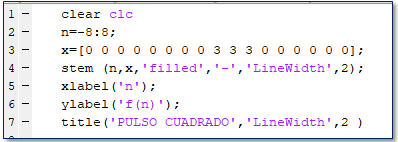
\includegraphics[scale=0.6]{../Imagenes de señales problema 2/Sin título.png} 
\end{figure}

\begin{figure}[h]
\centering
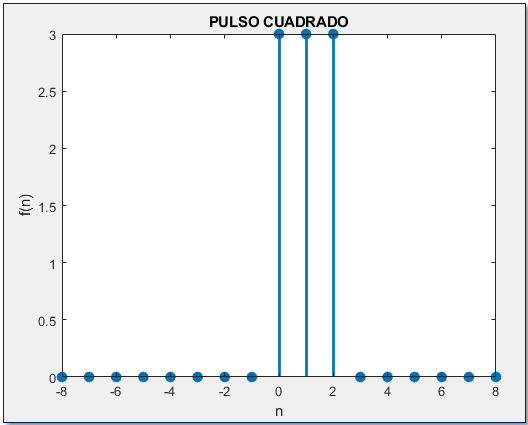
\includegraphics[scale=0.5]{../Imagenes de señales problema 2/pulso.png} 
\caption{Código en Matlab y gráfica de f[n]} 
\label{Gráfica_fn}
\end{figure}
$\bullet$Para la gráfica $g[n]=[1,2,3,2,1]$ , $-2\leq n\leq 2$, se utilizo la función stem de MATLAB para realizar un pulso rectangular consideramos en un intervalo de $[-8,8]$.

\begin{center}
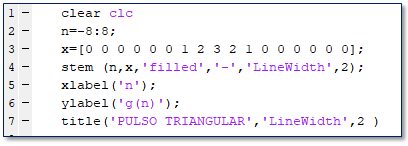
\includegraphics[scale=0.6]{../Imagenes de señales problema 2/sintutulo1.png}
\end{center}

\begin{figure}[h]
\centering
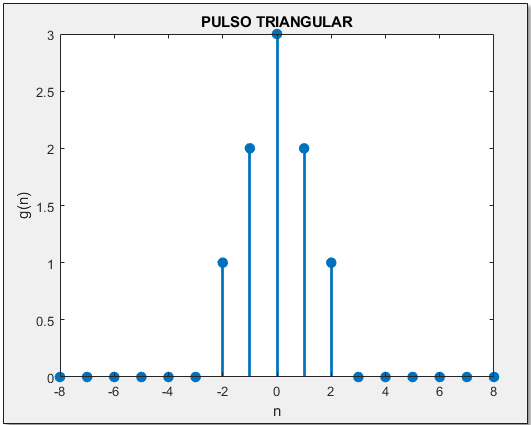
\includegraphics[scale=0.5]{../Imagenes de señales problema 2/triangulo.png} 
\caption{Código en Matlab y gráfica de g[n]} 
\label{Gráfica_gn}
\end{figure}
\newpage
$\bullet$Para la grafica $h[n]=(\frac{1}{2})^n$, se utilizo la funcion stem de MATLAB para realizar la amortiguación exponencial $[-8,8]$ con paso 1.
\begin{figure}[h]
\centering
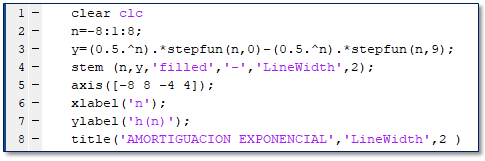
\includegraphics[scale=0.6]{../Imagenes de señales problema 2/titulo2.png} 
\label{Código_hn}
\end{figure}

\begin{figure}[h]
\centering
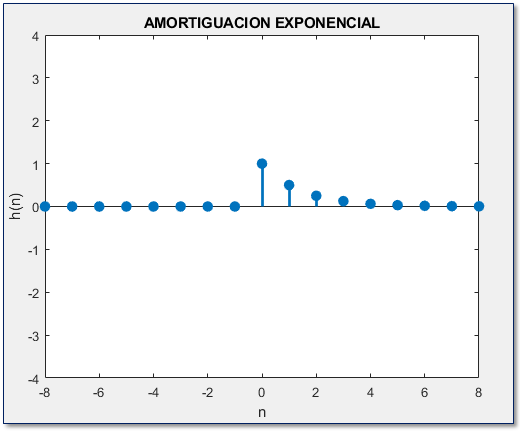
\includegraphics[scale=0.6]{../Imagenes de señales problema 2/expone.png} 
\caption{Código en Matlab y gráfica de h[n]}
\label{Gráfica_hn}
\end{figure}
	\item[\textbf{b)}]
	\textbf{Encuentre en términos de n y la señal escalón unitario las siguientes convoluciones:}\\
Como nos piden la convolución de dos señales discretas por conocimiento previo:
$$\boxed{y[n]=x[n]*h[n]=\sum_{k=-\infty}^{\infty}x[k]h[n-k]}$$
$\bullet$ Hallamos la convolución de $f[n]*g[n]$ con la formula previa hallada.
$$n<-2 \rightarrow y[n]=0$$
$$n=-2 \rightarrow y[n]=\sum_{k=-\infty}^{\infty}f[k]g[n-k]=f[0]g[-2]=(3)(1)=3$$
$$n=-1 \rightarrow y[n]=\sum_{k=-\infty}^{\infty}f[k]g[n-k]=f[0]g[-1]+f[1]g[-2]=9$$
$$n=0 \rightarrow y[n]=\sum_{k=-\infty}^{\infty}f[k]g[n-k]=f[0]g[n]+f[1]g[-1]+f[2]g[-2]=18$$
$$n=1 \rightarrow y[n]=\sum_{k=-\infty}^{\infty}f[k]g[n-k]=f[0]g[1]+f[1]g[0]+f[2]g[-1]=21$$
$$n=2 \rightarrow y[n]=\sum_{k=-\infty}^{\infty}f[k]g[n-k]=f[0]g[2]+f[1]g[1]+f[2]g[0]=18$$
$$n=3 \rightarrow y[n]=\sum_{k=-\infty}^{\infty}f[k]g[n-k]=f[1]g[2]+f[2]g[1]=9$$\\
$$n=4 \rightarrow y[n]=\sum_{k=-\infty}^{\infty}f[k]g[n-k]=f[2]g[2]=3$$\\
$$n>4 \rightarrow y[n]=0$$
\begin{equation*}
y[n]=f[n]*g[n] =
\begin{cases}
0 & \text{si $n<-2 $}\\
3 & \text{si $n= -2$}\\
9 & \text{si $n= -1$}\\
18 & \text{si $n= 0$}\\
21 & \text{si $n= 1$}\\
18 & \text{si $n= 2$}\\
9 & \text{si $n= 3$}\\
3 & \text{si $n=4$}\\
0 & \text{si $n>4$}
\end{cases}
\end{equation*}\\
\textbf{Expresamos en n y escalón unitario la señal:}
$$\boxed{y[n]=3u[n+2]+6u[n+1]+9u[n]+3u[n-1]-3u[n-2]-9u[n-3]-6u[n-4]-3u[n-5]}$$

$\bullet$ Hallamos la convolución de $f[n]*h[n]$ con la formula previa hallada.
$$f[n]*h[n]=\sum_{k=-\infty}^{\infty}f[k]h[n-k]$$
$$n<0 \rightarrow y[n]=0$$
$$n=0 \rightarrow y[n]=\sum_{k=-\infty}^{\infty}f[k]h[n-k]=f[0]h[0]=3$$
$$n=1 \rightarrow y[n]=\sum_{k=-\infty}^{\infty}f[k]h[n-k]=f[0]h[1]+f[1]h[0]=\frac{9}{2}$$
$$n=2 \rightarrow y[n]=\sum_{k=-\infty}^{\infty}f[k]h[n-k]=f[0]h[2]+f[1]h[1]+f[2]h[0]=\frac{21}{4}$$
$$n=3 \rightarrow y[n]=\sum_{k=-\infty}^{\infty}f[k]h[n-k]=f[0]h[3]+f[1]h[2]+f[2]h[1]=\frac{21}{8}$$
$$n=4 \rightarrow y[n]=\sum_{k=-\infty}^{\infty}f[k]h[n-k]=f[0]h[4]+f[1]h[3]+f[2]h[2]=\frac{21}{16}$$
$$n=5 \rightarrow y[n]=\sum_{k=-\infty}^{\infty}f[k]h[n-k]=f[0]h[5]+f[1]h[4]+f[2]h[3]=\frac{21}{32}$$
$$n=6 \rightarrow y[n]=\sum_{k=-\infty}^{\infty}f[k]h[n-k]=f[0]h[6]+f[1]h[5]+f[2]h[4]=\frac{21}{64}$$
$$n=7 \rightarrow y[n]=\sum_{k=-\infty}^{\infty}f[k]h[n-k]=f[0]h[7]+f[1]h[6]+f[2]h[5]=\frac{21}{128}$$
$$n=8 \rightarrow y[n]=\sum_{k=-\infty}^{\infty}f[k]h[n-k]=f[0]h[8]+f[1]h[7]+f[2]h[6]=\frac{21}{256}$$
$$n=9 \rightarrow y[n]=\sum_{k=-\infty}^{\infty}f[k]h[n-k]=f[1]h[8]+f[2]h[7]=\frac{9}{256}$$
$$n=10 \rightarrow y[n]=\sum_{k=-\infty}^{\infty}f[k]h[n-k]=f[2]h[8]=\frac{3}{256}$$
$$n>10 \rightarrow y[n]=\sum_{k=-\infty}^{\infty}f[k]h[n-k]=0$$
\begin{equation*}
y[n]=f[n]*h[n] =
\begin{cases}
0 & \text{si $n<0 $}\\
3 & \text{si $n= 0$}\\
\frac{9}{2} & \text{si $n= 1$}\\
\frac{21}{4} & \text{si $n= 2$}\\
\frac{21}{8} & \text{si $n= 3$}\\
\frac{21}{16} & \text{si $n= 4$}\\
\frac{21}{32} & \text{si $n= 5$}\\
\frac{21}{64} & \text{si $n=6$}\\
\frac{21}{128} & \text{si $n=7$}\\
\frac{21}{256} & \text{si $n=8$}\\
\frac{9}{256} & \text{si $n=9$}\\
\frac{3}{256} & \text{si $n=10$}\\
0 & \text{si $n>10$}
\end{cases}
\end{equation*}\\
\textbf{Expresamos en n y escalón unitario la señal:}
$$\boxed{y[n]=(0.5)^n(3u[n]+6u[n-1]+12u[n-2]-12u[n-9])-(0.5)^8(6u[n-10]-3u[n-11])}$$
$\bullet$ Hallamos la convolución de $g[n]*h[n]$ con la formula previa hallada.
$$g[n]*h[n]=\sum_{k=-\infty}^{\infty}g[k]h[n-k]$$
$$n<-2 \rightarrow y[n]=0 $$
$$n=-2 \rightarrow y[n]=\sum_{k=-\infty}^{\infty}g[k]h[n-k]=g[-2]h[0]=1 $$
$$n=-1 \rightarrow y[n]= \sum_{k=-\infty}^{\infty}g[k]h[n-k]=g[-1]h[0]+g[-2]h[1]=\frac{5}{2} $$
$$n=0 \rightarrow y[n]= \sum_{k=-\infty}^{\infty}g[k]h[n-k]=g[-2]h[2]+g[-1]h[1]+g[0]h[0]=\frac{17}{4} $$
$$n=1 \rightarrow y[n]= \sum_{k=-\infty}^{\infty}g[k]h[n-k]=g[-2]h[3]+g[-1]h[2]+g[0]h[1]+g[1]h[0]=\frac{33}{8} $$
$$n=2 \rightarrow y[n]= \sum_{k=-\infty}^{\infty}g[k]h[n-k]=g[-2]h[4]+g[-1]h[3]+g[0]h[2]+g[1]h[1]+g[2]h[0]=\frac{49}{16} $$
$$n=3 \rightarrow y[n]= \sum_{k=-\infty}^{\infty}g[k]h[n-k]=g[-2]h[5]+g[-1]h[4]+g[0]h[3]+g[1]h[2]+g[2]h[1] =\frac{49}{32}$$
$$n=4 \rightarrow y[n]= \sum_{k=-\infty}^{\infty}g[k]h[n-k]=g[-2]h[6]+g[-1]h[5]+g[0]h[4]+g[1]h[3]+g[2]h[2]=\frac{49}{64} $$
$$n=5 \rightarrow y[n]= \sum_{k=-\infty}^{\infty}g[k]h[n-k]=g[-2]h[7]+g[-1]h[6]+g[0]h[5]+g[1]h[4]+g[2]h[3]=\frac{49}{128} $$
$$n=6 \rightarrow y[n]= \sum_{k=-\infty}^{\infty}g[k]h[n-k]=g[-2]h[8]+g[-1]h[7]+g[0]h[6]+g[1]h[5]+g[2]h[4]=\frac{49}{256} $$
$$n=7 \rightarrow y[n]= \sum_{k=-\infty}^{\infty}g[k]h[n-k]=g[-1]h[8]+g[0]h[7]+g[1]h[6]+g[2]h[5]=\frac{3}{32} $$
$$n=8 \rightarrow y[n]= \sum_{k=-\infty}^{\infty}g[k]h[n-k]=g[0]h[8]+g[1]h[7]+g[2]h[6] =\frac{11}{256}$$
$$n=9 \rightarrow y[n]= \sum_{k=-\infty}^{\infty}g[k]h[n-k]=g[1]h[8]+g[2]h[7]=\frac{1}{64} $$
$$n=10 \rightarrow y[n]= \sum_{k=-\infty}^{\infty}g[k]h[n-k]=g[2]h[8]=\frac{1}{256}$$
$$n>10 \rightarrow y[n]=0 $$
\begin{equation*}
y[n]=g[n]*h[n] =
\begin{cases}
0 & \text{si $n<-2 $}\\
1 & \text{si $n= -2$}\\
\frac{5}{2} & \text{si $n= -1$}\\
\frac{17}{4} & \text{si $n= 0$}\\
\frac{33}{8} & \text{si $n= 1$}\\
\frac{49}{16} & \text{si $n= 2$}\\
\frac{49}{32} & \text{si $n= 3$}\\
\frac{49}{64} & \text{si $n=4$}\\
\frac{49}{128} & \text{si $n=5$}\\
\frac{49}{256} & \text{si $n=6$}\\
\frac{3}{32} & \text{si $n=7$}\\
\frac{11}{256} & \text{si $n=8$}\\
\frac{1}{64} & \text{si $n=9$}\\
\frac{1}{256} & \text{si $n=10$}\\
0 & \text{si $n>10$}
\end{cases}
\end{equation*}\\
\textbf{Expresamos en n y escalón unitario la señal:}
$$y[n]=(0.5)^n(u[n+2]+4u[n+1]+12u[n]+16u[n-1]+16u[n-2]-49u[n-7])$$ $$+(0.5)^5(3u[n-7]-3u[n-8])
+(0.5)^8(11u[n-8]-11u[n-9])$$ $$+(0.5)^6(u[n-9]-u[n-10])+(0.5)^8(u[n-10]-u[n-11])$$
	\end{enumerate}
	}}
	\section{{\large \textbf{(a)El esquema del diagrama de bloques,en el dominio de frecuencia compleja,que relaciona la entrada y salida de un sistema LTI causa,es el siguiente }}}{
	\large{
	\begin{enumerate}
	\item[\textbf{}]
	
	Determinar:\\
	$\bullet$ La función de transferencia $H(z)$ del mencionado sistema\\
	$\bullet$ La ecuación de diferencias de coeficientes constantes que representa al sistema\\
	$\bullet$ La respuesta al impulso $h[n]$\\
	\textbf{Solución:}\\
	\textbf{1er paso:}
	Encontrando las ecuaciones a partir del diagrama de bloques
	
	(a)\begin{center}
	$0.63Y_1(z)-1.6 Y_1(z) = X(z)-Y_1(z)Z^2$
	\end{center}
	\begin{eqnarray}
	\label{Y1Z}
		Y_1(z)=\dfrac{X(z)}{Z^2 - 1.6 Z+0.63}
	\end{eqnarray}
	(b)\begin{center}
	$Y(z)=4Y(z)-4Y_1(z)$
	\end{center}
	De (\ref{Y1Z})
	$$Y(z)=\dfrac{4 X(z) (Z-1)}{Z^2 - 1.6 Z+0.63}$$
	\textbf{Función transferencia:}
	\begin{center}
	$\therefore$ \boxed{H(z)=\dfrac{Y(z)}{X(z)}=\dfrac{4(Z-1)}{Z^2 - 1.6 Z+0.63}}
	\end{center}
    \textbf{2do paso:}\\
    Hallando la ecuación de diferencias de coeficientes constantes del sistema, a partir de \textbf{la función de transferencia}\\
    $$\dfrac{Y(z)}{X(z)}=\dfrac{4(Z-1)}{Z^2 - 1.6 Z+0.63}$$
    $$Z^2 Y(z)- 1.6 Z Y(z)+0.63 Y(z)=4(Z-1)X(z)$$
    Dividiendo entre $Z^2$ , para realizar la transformada inversa:
    $$Y(z)- 1.6 Z^{-1} Y(z)+0.63 Z^{-2} Y(z)=4 Z^{-1} X(z)-4 Z^{-2} X(z)$$
    Aplicamos la siguiente transformada inversa $x[n-a]=Z^{-1}\lbrace Z^{-a} X(z) \rbrace$\\
    \textbf{Ecuación de diferencias}
    \begin{center}
	$\therefore$ \boxed{y[n]-1.6 y[n-1]+0.63 y[n-2] = 4x[n]-4x[n-2]}
	\end{center}
	\newpage
	\textbf{3er paso:}\\
	Calculando la respuesta al impulso del sistema:
	Como la entrada es el impulso unitario, entonces $x[n]=\delta[n]$;por lo tanto, como $Z\lbrace \delta[n] \rbrace=X(z)=1$.Además, trabajaremos con la transformada Z.
	$$Y(z)=H(z)X(z)$$
	A partir de la función de transferencia, obtenemos $H(z)$.\\% Además $X(z)=1$
	$$Y(z)=H(z)X(z)$$
	$$Y(z)=\dfrac{4(Z-1)}{Z^2 - 1.6 Z+0.63}(1)$$
	$$Y(z)=2(\dfrac{-1}{Z-0.9}+\dfrac{3}{Z-0.7})$$
	Aplicando transformada inversa
	$$Z^{-1}\lbrace Y(z) \rbrace=2(-Z^{-1}\lbrace \dfrac{1}{Z-0.9} \rbrace +3 Z^{-1}\lbrace \dfrac{1}{z-0.7}\rbrace)$$
	\textbf{La respuesta al impulso al impulso unitario}
	\begin{center}
	$\therefore$ \boxed{h[n]=2(-(0.9)^{n-1}u_{(n-1)}+3(0.7)^{n-1}u_{(n-1)})}
	\end{center}
	\textbf{Importante:} Colocando como entrada la función impulso en el sistema\\
	Por medio del osciloscopio, se muestra la salida de la función impulso, en $Y(z)$
	\item[\textbf{b)}]
	El sistema global que se muestra en la siguiente figura, es el resultado de la combinación de 5 sistemas interconectados 
	\begin{center}
	$\therefore$ \boxed{h[n]=2(\delta[n]-\delta[n-1]+u[n-1]+(\frac{1}{2})^{n-1} u[n-1])}
	\end{center}
	\end{enumerate}
	}}
\end{document}









